%\VignetteIndexEntry{dartR_Introduction}
%\VignetteEngine{knitr::rmarkdown}
\usepackage[utf8]{inputenc}

\usepackage{tcolorbox}
\usepackage{graphicx}
\definecolor{light-gray}{gray}{0.95}

\usepackage{titling}
\pretitle{%
\begin{center}
\LARGE
\hfill 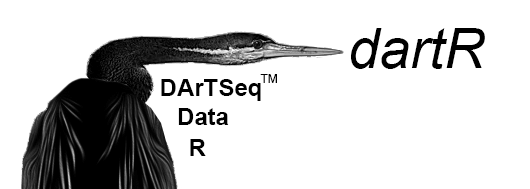
\includegraphics[width=15cm,height=8cm]{figures/dartRlogo.png}\\[\bigskipamount]
}
\posttitle{\end{center}}


\newenvironment{question}
  {\begin{tcolorbox}[width=\textwidth,colback={light-gray},title={
\includegraphics[height=1.5cm]{figures/dialog_question.png} Question},colbacktitle=light-gray, coltitle=black]    
  }
  {
  \end{tcolorbox}    
  }

\newenvironment{task}
  {\begin{tcolorbox}[width=\textwidth,colback={light-gray},title={
\includegraphics[height=1.5cm]{figures/penguin_task.png} Task},colbacktitle=light-gray, coltitle=black]    
  }
  {
  \end{tcolorbox}    
  }

\newenvironment{hint}
  {\begin{tcolorbox}[width=\textwidth,colback={light-gray},title={
\includegraphics[height=1.5cm]{figures/tux_info.png} Hint},colbacktitle=light-gray, coltitle=black]    
  }
  {
  \end{tcolorbox}    
  }







